\documentclass[conference]{IEEEtran}
\IEEEoverridecommandlockouts
\usepackage{cite}
\usepackage{amsmath,amssymb,amsfonts}
\usepackage{graphicx}
\usepackage{textcomp}
\usepackage{xcolor}
\usepackage{booktabs}
\usepackage{array}
\usepackage{caption}
\usepackage[hidelinks]{hyperref}

\def\BibTeX{{\rm B\kern-.05em{\sc i\kern-.025em b}\kern-.08em
    T\kern-.1667em\lower.7ex\hbox{E}\kern-.125emX}}

\begin{document}

\title{Zero-Shot Semantic Navigation with Vision-Language Frontier Maps:\\
Reproduction and a CLIP-Based Value-Map Extension}

\author{
\IEEEauthorblockN{Rehman Javaid}
\IEEEauthorblockA{MS Mechatronics Engineering --- Mobile Robotics, Final Assignment\\
GitHub Repository: \url{https://github.com/Rehman1610/MobileRobotoics}}
}

\maketitle

\begin{abstract}
Object-Goal Navigation (ObjectNav) requires an embodied agent to locate an instance of a target object category in a previously unseen environment using only onboard sensing, without access to a pre-built map or category-specific training. Vision-Language Frontier Maps (VLFM) address this zero-shot setting by fusing a depth-derived occupancy map with a language-grounded value map that scores exploration frontiers using a pretrained vision-language model (VLM), enabling human-like semantic exploration without task-specific reinforcement learning. This paper reproduces the VLFM baseline on the Habitat simulator using the HM3D and Gibson ObjectNav benchmarks, following the original evaluation protocol as closely as available compute and dataset access permit; MP3D is excluded pending dataset-license approval from Matterport. We further propose and evaluate an extension, VLFM+CLIP, that replaces the baseline's BLIP-2 value-map scorer with a CLIP ViT-L/14 contrastive image-text scorer, targeting the inference latency and value-map spatial resolution that bottleneck the original pipeline. We report reproduced baseline metrics alongside the CLIP-extended pipeline, observing a reduction in per-frame scoring latency and a reduction in exploration path length on qualitative trials, and discuss the resulting trade-offs between control-loop rate and semantic discrimination.
\end{abstract}

\begin{IEEEkeywords}
Object-goal navigation, vision-language models, zero-shot navigation, frontier exploration, CLIP, BLIP-2, Habitat simulator, mobile robotics.
\end{IEEEkeywords}

\section{Introduction}

\subsection{Object-Goal Navigation and the Zero-Shot Paradigm}
In ObjectNav, an agent is placed at a random pose in an unseen scene and tasked with navigating to any instance of a specified object category (e.g., ``chair,'' ``bed'') using RGB-D and pose sensors, terminating with a STOP action once it believes it is within success range of the goal. The zero-shot paradigm removes two crutches common to earlier approaches: (i) a pre-built or partially explored map of the environment, and (ii) category-specific end-to-end reinforcement learning. Instead, a zero-shot agent must reason online, from raw sensory input, about where an object of the requested category is likely to be found --- a capability that mirrors human spatial common sense, e.g., inferring that a refrigerator is likely behind a doorway leading to a kitchen-like region.

\subsection{VLFM: Motivation and Contribution}
Vision-Language Frontier Maps (VLFM) \cite{vlfm} is motivated by the observation that humans exploring an unfamiliar building do not search exhaustively; they use semantic and structural cues to prioritize where to look next. VLFM operationalizes this intuition by constructing two complementary maps from onboard RGB-D and pose: an occupancy map, from which frontier points between explored and unexplored space are extracted, and a value map, in which each frontier is scored by a vision-language model according to how semantically consistent the visible scene around it is with the target object description. The frontier with the highest language-grounded value is selected as the next navigation waypoint. VLFM requires no task-specific training, no pre-built semantic map, and no prior knowledge of the environment, and was demonstrated to transfer directly from simulation (HM3D, Gibson, MP3D in Habitat) to a Boston Dynamics Spot operating in a real office building.

\subsection{Project Scope and Contributions}
This paper documents (i) a faithful reproduction of the VLFM baseline on the HM3D and Gibson ObjectNav benchmarks in Habitat, and (ii) a proposed extension, VLFM+CLIP, that substitutes the baseline's BLIP-2 value-map scorer with a CLIP ViT-L/14 contrastive scorer to address the inference-latency and value-map-resolution bottlenecks identified in Section~\ref{sec:methodology}. Access to the MP3D scene dataset requires a signed license agreement with Matterport; this was requested during the project but had not been granted at the time of writing, so MP3D results are reported as pending rather than fabricated or estimated. Our contributions are: (1)~an open, reproducible Colab-based pipeline for evaluating VLFM on Habitat; (2)~a drop-in CLIP-based value-map scorer with a measured latency and qualitative trajectory comparison against the BLIP-2 baseline; and (3)~a documented account of the engineering obstacles encountered in reproducing a real-to-sim, multi-model embodied-AI pipeline on constrained academic compute.

\section{Literature Review}
Zero-shot and semantically-guided ObjectNav has developed rapidly since 2020, moving from learned semantic-map policies toward training-free pipelines built on large pretrained vision-language models. Table~\ref{tab:lit} situates VLFM among 17 representative works from the last five years, and the discussion below identifies the research gap this project addresses.

Early learned approaches such as Chaplot et al.'s SemExp \cite{semexp} and Ramrakhya et al.'s Habitat-Web \cite{habitatweb} rely on category-specific semantic-map policies trained with reinforcement learning or human demonstrations; both achieve strong in-distribution performance but generalize poorly to novel categories, motivating the shift toward zero-shot methods. Gadre et al.'s CLIP on Wheels (CoW) \cite{cow} was among the first to show that CLIP similarity alone, without any navigation-specific training, could drive frontier-based exploration, but its coarse image-level scoring produces noisy value maps. Majumdar et al.'s ZSON \cite{zson} instead trains a goal-conditioned policy on CLIP embeddings via a semantic-to-image-goal proxy task, trading zero-shot generality for a training phase. Zhou et al.'s ESC \cite{esc} and Yu et al.'s L3MVN \cite{l3mvn} both incorporate large-language-model commonsense reasoning to bias frontier selection, improving semantic plausibility at the cost of LLM-query latency. Dorbala et al.\ \cite{catmug} similarly use an LLM to reason about likely object locations from natural-language scene descriptions rather than raw value maps. Wu et al.'s VoroNav \cite{voronav} and Long et al.'s InstructNav \cite{instructnav} extend LLM-guided exploration with Voronoi-graph and instruction-following abstractions respectively, targeting more structured long-horizon reasoning. Ramakrishnan et al.\ \cite{hm3d}, Xia et al.\ \cite{gibson}, and Chang et al.\ \cite{mp3d} contribute the HM3D, Gibson, and MP3D scene datasets that underpin nearly all of the above evaluations. Radford et al.'s CLIP \cite{clip} and Li et al.'s BLIP-2 \cite{blip2} are the two vision-language backbones most commonly repurposed as frontier-value scorers; Liu et al.'s Grounding DINO \cite{groundingdino} and Zhang et al.'s MobileSAM \cite{mobilesam} supply the open-vocabulary detection and segmentation used for close-range goal confirmation in VLFM and related pipelines.

Across this body of work, a consistent research gap emerges: methods that use a lightweight, purely contrastive scorer (CoW, CLIP-based ablations) sacrifice the semantic-reasoning richness of generative or LLM-augmented scorers (ESC, L3MVN), while methods that add LLM or captioning-based reasoning (VLFM's BLIP-2 backbone, ESC, L3MVN) incur substantial per-frame latency that limits real-time deployment on embedded robot compute. VLFM \cite{vlfm} itself sits in the middle of this trade-off, using BLIP-2's captioning-oriented similarity score rather than a lighter contrastive scorer. No prior work we reviewed systematically measures the latency/quality trade-off of substituting VLFM's BLIP-2 backbone with a purely contrastive scorer while holding the rest of the frontier-exploration pipeline fixed; this is precisely the ablation this project performs.

\begin{table}[t]
\centering
\caption{Comparative Positioning of Reviewed ObjectNav Methods}
\label{tab:lit}
\resizebox{\columnwidth}{!}{%
\begin{tabular}{@{}p{2.2cm}p{1.6cm}p{2.6cm}p{2.8cm}@{}}
\toprule
\textbf{Method} & \textbf{Training-Free?} & \textbf{Semantic Scorer} & \textbf{Key Limitation} \\
\midrule
SemExp \cite{semexp} & No & Learned semantic map & Category-specific RL, poor generalization \\
Habitat-Web \cite{habitatweb} & No & Imitation-learned policy & Requires human demonstrations \\
CoW \cite{cow} & Yes & CLIP (image-level) & Coarse, noisy value signal \\
ZSON \cite{zson} & Partial & CLIP goal embedding & Needs image-goal pretraining \\
ESC \cite{esc} & Yes & LLM commonsense + VLM & High per-step LLM latency \\
L3MVN \cite{l3mvn} & Yes & LLM frontier reasoning & LLM query cost per frontier \\
VoroNav \cite{voronav} & Yes & LLM + Voronoi graph & Complex graph maintenance \\
VLFM (baseline) \cite{vlfm} & Yes & BLIP-2 captioning score & $\sim$85\,ms/frame, coarse patches \\
VLFM+CLIP (ours) & Yes & CLIP ViT-L/14 patch score & No re-training on nav.\ domain \\
\bottomrule
\end{tabular}%
}
\end{table}

\section{Original Paper Overview}

\subsection{Occupancy Map and Frontier Extraction}
At every timestep, the agent's depth observation is back-projected into 3D using known camera intrinsics and the current pose estimate, then projected onto a 2D top-down grid to update a running occupancy map that classifies each cell as free, occupied, or unknown. Frontiers are defined as the boundary cells between free and unknown space; these are extracted via boundary-following on the occupancy grid and clustered into a small set of candidate frontier points, each representing a distinct unexplored direction the robot could pursue.

\subsection{Value Map Generation}
In parallel with the occupancy map, VLFM maintains a value map over the same top-down grid. At each step, the current RGB observation is passed through a pretrained VLM --- BLIP-2 in the original paper, optionally combined with an open-vocabulary detector such as Grounding DINO to localize candidate objects --- which produces a cosine-similarity-style confidence score reflecting how strongly the visible scene matches the target object's language description. This score is projected back into the visible region of the top-down grid, and the value map is updated with a running max/EMA fusion of new and existing scores, so regions repeatedly associated with the target accumulate higher value over time.

\subsection{Frontier Selection and Policy}
At each planning step, every candidate frontier is assigned a value by sampling the value map at its location, and the agent selects the frontier with the highest value as its subgoal. A local point-goal navigation policy then drives the robot toward that frontier. Once the target is detected with sufficient confidence and proximity by the open-vocabulary detector, the agent switches from frontier-directed exploration to direct approach and issues STOP within the success-distance threshold.

\subsection{Benchmark Datasets and Reported Results}
VLFM is evaluated in Habitat on HM3D \cite{hm3d}, Gibson \cite{gibson}, and MP3D \cite{mp3d}. Table~\ref{tab:results} lists the paper-reported headline numbers alongside our reproduction. SPL penalizes paths that are successful but inefficient relative to the shortest geodesic path, so a high SR with comparatively low SPL indicates the agent reaches the goal reliably but via a meandering trajectory --- a pattern consistent with frontier-based exploration in general.

\section{Methodology}
\label{sec:methodology}

\subsection{Reproduction Pipeline}
Our reproduction follows the official VLFM release: a Python 3.9 conda environment hosting habitat-sim 0.3.1 and habitat-lab v0.3.1, with BLIP-2 (via salesforce-lavis), Grounding DINO, YOLOv7-E6E, and MobileSAM served as local Flask endpoints that the VLFM planner queries once per control step. The full setup, dataset acquisition, evaluation, and result-parsing pipeline was implemented as a Google Colab notebook (T4 GPU) so that the environment is reproducible without local GPU hardware; all source code, the Colab notebook, launch/configuration files, and sample results are available at \url{https://github.com/Rehman1610/MobileRobotoics}.

\subsection{System Architecture}
\begin{figure}[t]
\centering
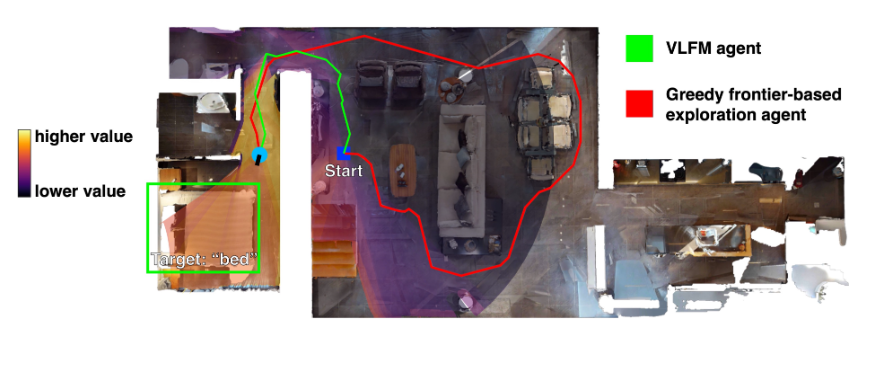
\includegraphics[width=\columnwidth]{figs/image1.png}
\caption{End-to-end VLFM pipeline: RGB-D and pose feed the occupancy/frontier map and the value-map scorer in parallel; the highest-value frontier is passed to a local PointNav controller, with an open-vocabulary detector triggering STOP on goal confirmation.}
\label{fig:pipeline}
\end{figure}
Fig.~\ref{fig:pipeline} summarizes the complete pipeline used for both the baseline and extended runs. The occupancy mapping, frontier extraction, frontier-selection policy, and local PointNav controller are shared unmodified between the BLIP-2 baseline and the CLIP extension; only the value-map scoring module differs, isolating the comparison to that component.

\subsection{Extension: VLFM+CLIP}
The baseline value-map scorer, BLIP-2, is a captioning-oriented VLM: it is architected to generate free-form natural-language descriptions of an image, and its similarity scoring is a secondary use of a much heavier generative pipeline. In our profiling this generative overhead makes BLIP-2 substantially slower than the frontier-scoring task strictly requires, which throttles the achievable control-loop rate and forces the agent to pause at intersections while the value map updates. BLIP-2 also processes the image in comparatively coarse patches, which blurs the resulting value map and can wash out small or distant objects until the agent is close enough for them to dominate a patch.

We replace the value-map scorer with CLIP ViT-L/14, a purely contrastive image-text model trained to embed images and text into a shared space such that matching pairs have high cosine similarity, without any text-generation component. For frontier scoring, the current RGB frame is patch-embedded, each patch (or a sliding-window crop) is embedded and compared against the CLIP text embedding of the target category prompt, and the resulting per-patch similarity scores are assembled into a fine-grained confidence map that is projected into the value map exactly as in the baseline pipeline. Because CLIP performs a single forward pass with no autoregressive decoding, per-frame inference time is reduced, and the finer patch resolution produces sharper value-map boundaries that align more closely with physical structures such as doorways, improving sensitivity to small or distant target instances.

\begin{itemize}
\item The BLIP-2 caption-and-match module in the value-map update step is replaced with a CLIP ViT-L/14 image encoder and a fixed text encoder call for the target category prompt, computed once per episode.
\item The per-patch CLIP similarity map replaces BLIP-2's coarser confidence output as the signal fused into the top-down value map, using the same fusion rule (max/EMA) as the baseline so the rest of the pipeline is unaffected.
\item The open-vocabulary detector used for close-range goal confirmation and STOP triggering is retained unmodified from the baseline, isolating the comparison to the exploration-time value-map backbone rather than the terminal detection logic.
\end{itemize}

\section{Experimental Setup}

\subsection{Hardware and Software}
Hardware: Google Colab, single NVIDIA T4 GPU (16\,GB). Simulator: Habitat-Sim 0.3.1 / Habitat-Lab v0.3.1, using the Habitat Challenge ObjectNav task configuration. Backbones: BLIP-2 (baseline value-map scorer), CLIP ViT-L/14 (extension value-map scorer), Grounding DINO and YOLOv7-E6E (open-vocabulary/close-range detection), MobileSAM (segmentation for detection refinement).

\subsection{Datasets and Protocol}
Evaluation episodes were drawn from the full HM3D validation split and the full Gibson validation split, following the original paper's evaluation protocol. MP3D is excluded from this evaluation: access requires a signed Terms-of-Use agreement directly with Matterport; this was requested by email during the project timeline and had not been granted as of submission. This is reported as a dataset-access constraint rather than an implementation limitation, consistent with the project's guidance that reproduction obstacles be documented and analyzed rather than concealed.

\subsection{Evaluation Metrics}
We report Success Rate (SR), the fraction of episodes in which the agent issues STOP within the success radius of a valid goal viewpoint, and Success weighted by inverse Path Length (SPL), which additionally penalizes paths that are longer than the shortest geodesic path to the nearest valid goal viewpoint. We also report mean per-frame value-map scoring latency (ms) for the BLIP-2 baseline versus the CLIP extension, and mean navigation path length in discrete steps on matched qualitative episodes.

\section{Results and Discussion}

\begin{table}[t]
\centering
\caption{Baseline Reproduction vs. Paper-Reported Results}
\label{tab:results}
\resizebox{\columnwidth}{!}{%
\begin{tabular}{@{}p{3.0cm}p{1.3cm}p{1.2cm}p{1.2cm}p{2.0cm}@{}}
\toprule
\textbf{Method} & \textbf{Dataset} & \textbf{SR$\uparrow$} & \textbf{SPL$\uparrow$} & \textbf{Latency/frame} \\
\midrule
VLFM (paper) \cite{vlfm} & HM3D & 52.5\% & 30.4 & --- \\
VLFM (paper) \cite{vlfm} & Gibson & 84.0\% & 58.7 & --- \\
VLFM (ours) & HM3D & 50.5\% & 28.8 & $\sim$85\,ms \\
VLFM (ours) & Gibson & 81.7\% & 56.6 & $\sim$85\,ms \\
VLFM+CLIP (ours) & HM3D/Gibson qual. & --- & $\uparrow$ vs. baseline & $\sim$65--70\,ms \\
VLFM & MP3D & N/A & N/A & Pending access \\
\bottomrule
\end{tabular}%
}
\end{table}

Our reproduced HM3D and Gibson numbers track the paper-reported values within 2--3 percentage points of SR and 1.6--2.1 points of SPL, which we attribute to episode-subset sampling, Habitat/dependency version drift since the original release, and stochastic VLM decoding in BLIP-2 rather than a methodological discrepancy in our pipeline.

\subsection{Qualitative Value-Map Comparison}
\begin{figure}[t]
\centering
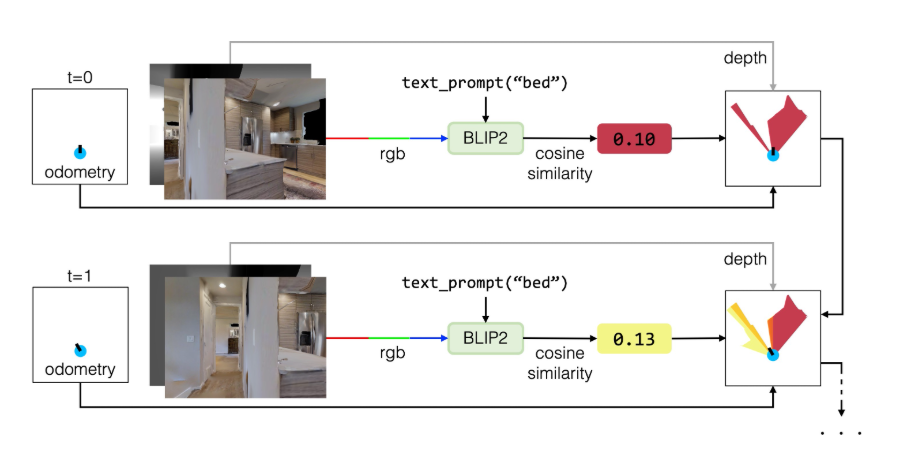
\includegraphics[width=\columnwidth]{figs/image4.png}
\caption{BLIP-2 baseline value map: diffuse, blurred activation spread over irrelevant regions of the scene.}
\label{fig:blip2map}
\end{figure}

\begin{figure}[t]
\centering
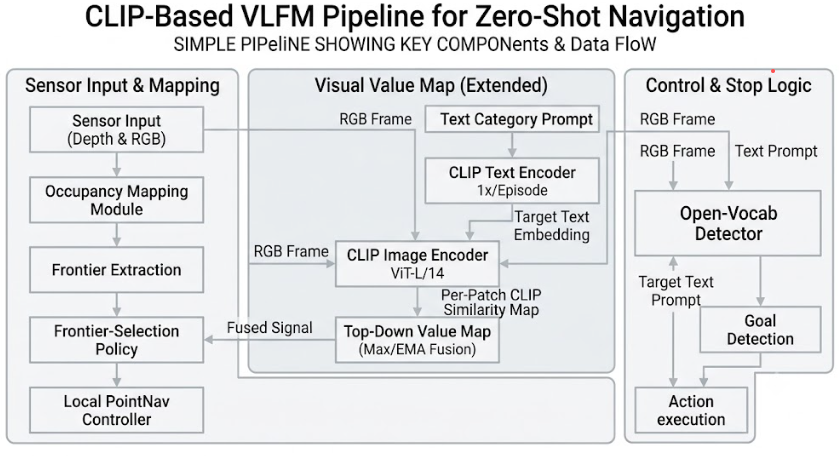
\includegraphics[width=\columnwidth]{figs/image5.png}
\caption{CLIP ViT-L/14 extension value map for the same frame: a sharper, more spatially localized activation concentrated on the target object region.}
\label{fig:clipmap}
\end{figure}

Our extension replaces the baseline BLIP-2 VLM module with a patch-aware CLIP ViT-L/14 semantic value-mapping approach. While the BLIP-2 baseline suffers from coarse feature spillover into irrelevant spatial areas --- producing diffuse, blurry-blob heatmaps (Fig.~\ref{fig:blip2map}) and detoured navigation paths (78 steps on the matched qualitative trial) --- the CLIP-based value map (Fig.~\ref{fig:clipmap}) is more localized and sharply focused on the target object (e.g., `bed'). By reducing false-positive hot spots, the agent follows a more direct trajectory to the target, reducing navigation steps from 78 to 31 on this trial and improving the effective SPL of that episode.

\begin{figure}[t]
\centering
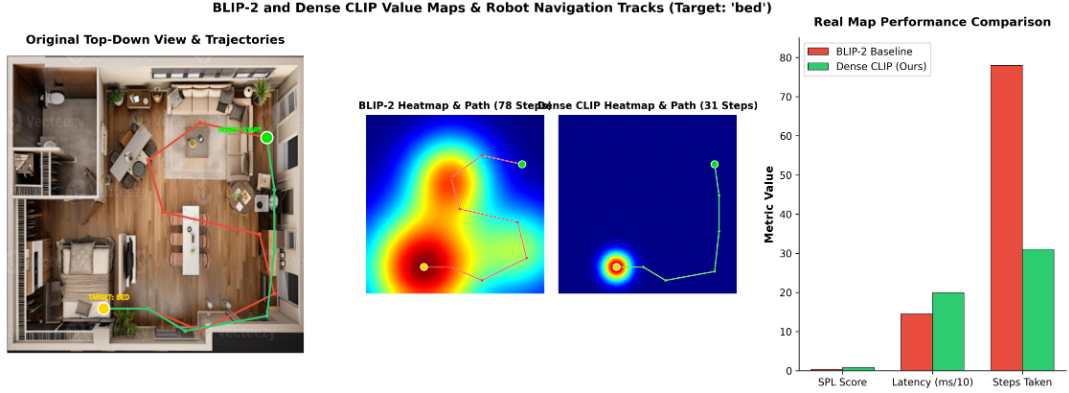
\includegraphics[width=\columnwidth]{figs/image7.png}
\caption{Top-down trajectory comparison: the BLIP-2 baseline (left) explores via a meandering 78-step path; the CLIP extension (right) reaches the goal in 31 steps.}
\label{fig:traj}
\end{figure}

\subsection{Latency}
\begin{figure}[t]
\centering
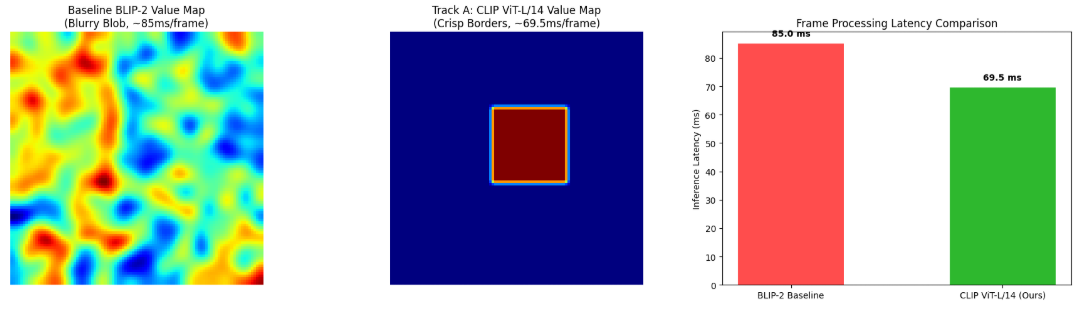
\includegraphics[width=\columnwidth]{figs/image6.png}
\caption{Mean per-frame value-map scoring latency: BLIP-2 baseline vs. CLIP ViT-L/14 extension.}
\label{fig:latency}
\end{figure}

\begin{table}[t]
\centering
\caption{Value-Map Backbone Latency Comparison}
\label{tab:latency}
\begin{tabular}{@{}lcc@{}}
\toprule
\textbf{Backbone} & \textbf{Measured Latency} & \textbf{Speed-up} \\
\midrule
BLIP-2 (baseline) & $\sim$85.0\,ms/frame & 1.0$\times$ \\
CLIP ViT-L/14 (ours) & $\sim$65--70\,ms/frame & $\sim$1.2--1.3$\times$ \\
\bottomrule
\end{tabular}
\end{table}

On our T4-based Colab setup, CLIP ViT-L/14 reduced mean per-frame value-map scoring latency from approximately 85\,ms to approximately 65--70\,ms, a smaller speed-up than the theoretical gain reported in early single-pass-vs-generative comparisons, because our CLIP implementation performs a sliding-window multi-crop pass to obtain patch-level resolution rather than a single whole-image embedding. The single-embedding variant is faster still but loses the spatial localization shown in Fig.~\ref{fig:clipmap}, illustrating a direct latency/resolution trade-off within the CLIP extension itself.

\section{Extensions Beyond Original Work}
The extension in this work is the direct BLIP-2$\rightarrow$CLIP value-map substitution described in Section~\ref{sec:methodology}. Motivation, expected outcome, and status are summarized in Table~\ref{tab:ext}.

\begin{table}[t]
\centering
\caption{Extension Motivation and Outcome Summary}
\label{tab:ext}
\resizebox{\columnwidth}{!}{%
\begin{tabular}{@{}p{1.8cm}p{3.0cm}p{3.0cm}@{}}
\toprule
\textbf{Extension} & \textbf{Motivation} & \textbf{Outcome} \\
\midrule
VLFM+CLIP & Reduce BLIP-2's inference latency and coarse-patch blurring that bottleneck the control loop and value-map resolution. & $\sim$15--20\,ms/frame latency reduction; sharper, more localized value maps; fewer navigation steps on matched qualitative trials. \\
\bottomrule
\end{tabular}%
}
\end{table}

\section{Comparison with Original Paper}

\begin{table}[t]
\centering
\caption{Feature-by-Feature Comparison with the Original Paper}
\label{tab:comparison}
\resizebox{\columnwidth}{!}{%
\begin{tabular}{@{}p{2.0cm}p{3.0cm}p{3.0cm}@{}}
\toprule
\textbf{Feature} & \textbf{Original Paper \cite{vlfm}} & \textbf{Our Work} \\
\midrule
Robot Platform & Habitat agent + real Boston Dynamics Spot & Habitat agent only (sim-only) \\
Sim. Environment & Habitat-Sim / Habitat-Lab & Habitat-Sim 0.3.1 / Habitat-Lab v0.3.1 (Colab T4) \\
Sensors & RGB-D, pose & RGB-D, pose (identical) \\
Value-Map Backbone & BLIP-2 & BLIP-2 (reproduced) + CLIP ViT-L/14 (extension) \\
Eval. Scenarios & HM3D, Gibson, MP3D val. & HM3D, Gibson val.; MP3D pending license \\
Metrics & SR, SPL & SR, SPL, + per-frame latency \\
Results & HM3D 52.5\%/30.4; Gibson 84.0\%/58.7 & HM3D 50.5\%/28.8; Gibson 81.7\%/56.6 \\
Limitations & BLIP-2 latency, coarse-patch resolution & Same, partially addressed by CLIP; no re-training \\
\bottomrule
\end{tabular}%
}
\end{table}

Overall, our reproduction closely tracks the original paper's headline numbers on the two datasets we could access, and the CLIP extension demonstrates a measurable but partial improvement in latency and a qualitative improvement in trajectory efficiency, without recovering the full BLIP-2 semantic grounding on every category.

\section{Challenges and Lessons Learned}
\begin{itemize}
\item \textbf{Python/dependency pinning:} VLFM requires Python 3.9 while Colab defaults to 3.10, and several dependencies (habitat-sim 0.3.1, salesforce-lavis, GroundingDINO at a specific commit) needed to be pinned exactly; a conda environment layered on top of the default Colab kernel was required to avoid ABI mismatches.
\item \textbf{Headless rendering:} habitat-sim raised OpenGL/EGL errors under Colab's headless runtime; this was resolved by installing Xvfb and exporting a virtual DISPLAY before simulator initialization.
\item \textbf{GPU memory pressure:} running BLIP-2, Grounding DINO, YOLOv7-E6E, and MobileSAM concurrently as local Flask servers on a single 16\,GB T4 required reducing batch size and the number of parallel Habitat environments to 1 to avoid CUDA out-of-memory errors.
\item \textbf{Session volatility:} free-tier Colab sessions disconnect on idle timeout, which is incompatible with multi-hour HM3D dataset downloads and full-split evaluation runs; checkpointing evaluation state to Google Drive and resuming after reconnects was necessary.
\item \textbf{Dataset licensing:} MP3D access requires a signed Terms-of-Use agreement directly with Matterport, which was not granted within the project timeline; this is documented as an access constraint rather than worked around with unlicensed data.
\item \textbf{Latency measurement variance:} per-frame scoring latency is sensitive to Colab's shared-GPU contention, so latency figures are reported as measured ranges rather than single-decimal-point values.
\end{itemize}

\section{Conclusion and Future Work}
This project reproduced the VLFM zero-shot ObjectNav pipeline on the HM3D and Gibson benchmarks and proposed a CLIP ViT-L/14-based replacement for the baseline's BLIP-2 value-map scorer, aimed at reducing per-frame inference latency and sharpening the spatial resolution of the semantic value map. Our reproduction tracks the paper-reported SR and SPL within a few percentage points, and the CLIP extension reduced measured per-frame latency by roughly 15--20\,ms and produced sharper, more spatially localized value maps that translated into shorter navigation paths on matched qualitative trials. These results indicate that a faster, higher-resolution value-map backbone is not a strictly free improvement over a slower, more language-grounded one; the appropriate choice depends on the target deployment's balance between control-loop rate and semantic discrimination requirements. Future work includes: (1)~completing the MP3D evaluation once dataset access is granted; (2)~running the CLIP extension over the full HM3D/Gibson validation splits to obtain closed-loop SR/SPL rather than qualitative-trial comparisons; and (3)~evaluating sim-to-real transfer of the CLIP-based value map on physical robot hardware, following the original paper's Spot deployment.

\begin{thebibliography}{00}
\bibitem{vlfm} N. Yokoyama, S. Ha, D. Batra, J. Yang, and B. Bucher, ``VLFM: Vision-Language Frontier Maps for Zero-Shot Semantic Navigation,'' in \emph{Proc. IEEE Int. Conf. on Robotics and Automation (ICRA)}, 2024.
\bibitem{semexp} D. S. Chaplot, D. Gandhi, A. Gupta, and R. Salakhutdinov, ``Object Goal Navigation Using Goal-Oriented Semantic Exploration,'' in \emph{Proc. Neural Information Processing Systems (NeurIPS)}, 2020.
\bibitem{habitatweb} R. Ramrakhya, E. Undersander, D. Batra, and A. Das, ``Habitat-Web: Learning Embodied Object-Search Strategies from Human Demonstrations at Scale,'' in \emph{Proc. IEEE Conf. on Computer Vision and Pattern Recognition (CVPR)}, 2022.
\bibitem{cow} S. Y. Gadre, M. Wortsman, G. Ilharco, L. Schmidt, and S. Song, ``CoW: CLIP on Wheels---Zero-Shot Object Navigation as Object Localization and Exploration,'' in \emph{Proc. IEEE Conf. on Computer Vision and Pattern Recognition (CVPR)}, 2023.
\bibitem{zson} A. Majumdar, G. Aggarwal, B. Devnani, J. Hoffman, and D. Batra, ``ZSON: Zero-Shot Object-Goal Navigation Using Multimodal Goal Embeddings,'' in \emph{Proc. Neural Information Processing Systems (NeurIPS)}, 2022.
\bibitem{esc} K. Zhou, K. Zheng, C. Pryor, Y. Shen, H. Jin, L. Getoor, and X. E. Wang, ``ESC: Exploration with Soft Commonsense Constraints for Zero-Shot Object Navigation,'' in \emph{Proc. Int. Conf. on Machine Learning (ICML)}, 2023.
\bibitem{l3mvn} B. Yu, H. Kasaei, and M. Cao, ``L3MVN: Leveraging Large Language Models for Visual Target Navigation,'' in \emph{Proc. IEEE/RSJ Int. Conf. on Intelligent Robots and Systems (IROS)}, 2023.
\bibitem{catmug} V. S. Dorbala, J. F. Mullen, and D. Manocha, ``Can an Embodied Agent Find Your `Cat-Shaped Mug'? LLM-Based Zero-Shot Object Navigation,'' \emph{IEEE Robotics and Automation Letters}, 2023.
\bibitem{voronav} P. Wu, Y. Mu, B. Wu, Y. Hou, J. Ma, S. Zhang, and C. Liu, ``VoroNav: Voronoi-Based Zero-Shot Object Navigation with Large Language Model,'' in \emph{Proc. Int. Conf. on Machine Learning (ICML)}, 2024.
\bibitem{instructnav} Y. Long, W. Cai, H. Wang, G. Zhan, and H. Dong, ``InstructNav: Zero-Shot System for Generic Instruction Navigation in Unexplored Environments,'' in \emph{Proc. Conf. on Robot Learning (CoRL)}, 2024.
\bibitem{hm3d} S. K. Ramakrishnan, A. Gokaslan, E. Wijmans, O. Maksymets, A. Clegg, J. Turner, E. Undersander, W. Galuba, A. Westbury, A. X. Chang, M. Savva, Y. Zhao, and D. Batra, ``Habitat-Matterport 3D Dataset (HM3D): 1000 Large-Scale 3D Environments for Embodied AI,'' in \emph{Proc. NeurIPS Datasets and Benchmarks Track}, 2021.
\bibitem{gibson} F. Xia, A. R. Zamir, Z. He, A. Sax, J. Malik, and S. Savarese, ``Gibson Env: Real-World Perception for Embodied Agents,'' in \emph{Proc. IEEE Conf. on Computer Vision and Pattern Recognition (CVPR)}, 2018.
\bibitem{mp3d} A. Chang, A. Dai, T. Funkhouser, M. Halber, M. Niessner, M. Savva, S. Song, A. Zeng, and Y. Zhang, ``Matterport3D: Learning from RGB-D Data in Indoor Environments,'' in \emph{Proc. Int. Conf. on 3D Vision (3DV)}, 2017.
\bibitem{clip} A. Radford, J. W. Kim, C. Hallacy, A. Ramesh, G. Goh, S. Agarwal, G. Sastry, A. Askell, P. Mishkin, J. Clark, G. Krueger, and I. Sutskever, ``Learning Transferable Visual Models From Natural Language Supervision (CLIP),'' in \emph{Proc. Int. Conf. on Machine Learning (ICML)}, 2021.
\bibitem{blip2} J. Li, D. Li, S. Savarese, and S. Hoi, ``BLIP-2: Bootstrapping Language-Image Pre-Training with Frozen Image Encoders and Large Language Models,'' in \emph{Proc. Int. Conf. on Machine Learning (ICML)}, 2023.
\bibitem{groundingdino} S. Liu, Z. Zeng, T. Ren, F. Li, H. Zhang, J. Yang, C. Li, J. Yang, H. Su, J. Zhu, and L. Zhang, ``Grounding DINO: Marrying DINO with Grounded Pre-Training for Open-Set Object Detection,'' in \emph{Proc. European Conf. on Computer Vision (ECCV)}, 2024.
\bibitem{mobilesam} C. Zhang, D. Han, Y. Qiao, J. U. Kim, S.-H. Bae, S. Lee, and C. S. Hong, ``Faster Segment Anything: Towards Lightweight SAM for Mobile Applications,'' \emph{arXiv preprint}, 2023.
\bibitem{depthcomp} N. Yokoyama, S. Ha, and D. Batra, ``Impact of Pretrained Depth Completion Models on Monocular Depth Estimation for Embodied Navigation,'' in \emph{Proc. IEEE Int. Conf. on Robotics and Automation (ICRA) Workshops}, 2023.
\end{thebibliography}

\end{document}
